\CWHeader{Лабораторная работа \textnumero 3.2}
\CWProblem{
Реализовать метод стрельбы и конечно-разностный метод решения краевой задачи для ОДУ в виде программ. 
С использованием разработанного программного обеспечения решить краевую задачу для обыкновенного дифференциального уравнения 
2-го порядка на указанном отрезке. Оценить погрешность численного решения с использованием метода Рунге – Ромберга и путем сравнения с точным решением. 

$$
\begin{cases}
    y'' + 4xy' + (4x^2 + 2)y = 0 \\
    y(0) = 0 \\
    y(1) = \frac{2}{e} \\
\end{cases}
$$

Точное решение:
$$
y(x) = (1 + x) e^{-x^2}
$$

Краевые условия не совпадают с вариантом, так как были изменены преподавателем.
}

\section*{Описание}

\subsection*{Метод стрельбы}
Суть метода заключается в сведении краевой задачи к последовательности задач Коши. Рассмотрим краевую задачу:

\begin{equation}
    y'' = f(x, y, y'), \quad y(a) = y_0, \quad y(b) = y_1
    \tag{4.28-4.29}
\end{equation}

\subsubsection*{Алгоритм метода}
\begin{enumerate}
    \item Заменяем второе граничное условие на начальное условие для производной:
    \begin{equation}
        y(a) = y_0, \quad y'(a) = \eta
        \label{eq:initial_condition}
    \end{equation}
    
    \item Решаем задачу Коши для пробного значения параметра $\eta_0$
    
    \item Вычисляем отклонение полученного решения от целевого условия:
    \begin{equation}
        \Delta(\eta) = y(b, y_0, \eta) - y_1
        \label{eq:deviation}
    \end{equation}
    
    \item Корректируем параметр $\eta$ по методу секущих:
    \begin{equation}
        \eta_{j+2} = \eta_{j+1} - \frac{\eta_{j+1} - \eta_j}{\Delta(\eta_{j+1}) - \Delta(\eta_j)} \Delta(\eta_{j+1})
        \label{eq:secant_method}
    \end{equation}
    
    \item Повторяем процесс, пока $|\Delta(\eta)|$ не станет меньше заданной точности $\epsilon$
\end{enumerate}


\subsection*{Конечно-разностный метод}
Для линейного уравнения:
\begin{equation}
    y'' + p(x)y' + q(x)y = f(x), \quad y(a)=y_0, \quad y(b)=y_1
    \tag{4.35-4.36}
\end{equation}

\subsubsection*{Алгоритм}
\begin{enumerate}
    \item Аппроксимируем производные:
    \begin{align}
        y_k' &\approx \frac{y_{k+1} - y_{k-1}}{2h} \\
        y_k'' &\approx \frac{y_{k+1} - 2y_k + y_{k-1}}{h^2}
        \tag{4.37}
    \end{align}
    
    \item Получаем систему:
    \begin{equation}
        \frac{y_{k+1} - 2y_k + y_{k-1}}{h^2} + p_k \frac{y_{k+1} - y_{k-1}}{2h} + q_k y_k = f_k
        \tag{4.38}
    \end{equation}
    
    \item Приводим к трёхдиагональной форме:
    \begin{equation}
        A_k y_{k-1} + B_k y_k + C_k y_{k+1} = D_k
        \tag{4.39}
    \end{equation}
\end{enumerate}

\section*{Исходный код}

\begin{minted}{java}
package cat.mood;

import java.util.Arrays;

public class BoundaryValueProblemSolver {

    interface ODEFunction {
        double f(double x, double y, double z); // z = y'
        double g(double x, double y, double z); // z' = y''
    }

    interface ExactSolution {
        double y(double x);
        double z(double x);
    }

    // Метод стрельбы для краевых условий y(a) = ya, y(b) = yb
    public static double[][] shootingMethod(ODEFunction ode, ExactSolution exact,
                                            double a, double b, double ya, double yb,
                                            double h, double eps) {
        // Начальные предположения для y'(a)
        double eta0 = 1.0;
        double eta1 = 0.5;

        // Первое приближение
        double[][] sol0 = rungeKutta4System(ode, a, ya, eta0, h, (int)((b-a)/h));
        double phi0 = sol0[sol0.length-1][1] - yb;

        // Второе приближение
        double[][] sol1 = rungeKutta4System(ode, a, ya, eta1, h, (int)((b-a)/h));
        double phi1 = sol1[sol1.length-1][1] - yb;

        // Метод секущих для нахождения правильного eta
        double eta = eta1;
        double phi = phi1;
        int iterations = 0;

        while (Math.abs(phi) > eps && iterations < 100) {
            double etaNew = eta1 - (eta1 - eta0)/(phi1 - phi0)*phi1;

            eta0 = eta1;
            eta1 = etaNew;
            phi0 = phi1;

            double[][] solNew = rungeKutta4System(ode, a, ya, eta1, h, (int)((b-a)/h));
            phi1 = solNew[solNew.length-1][1] - yb;

            eta = eta1;
            phi = phi1;
            iterations++;
        }

        // Финальное решение
        double[][] finalSolution = rungeKutta4System(ode, a, ya, eta, h, (int)((b-a)/h));

        // Добавляем точные значения и погрешности
        double[][] result = new double[finalSolution.length][5];
        for (int i = 0; i < finalSolution.length; i++) {
            result[i][0] = finalSolution[i][0]; // x
            result[i][1] = finalSolution[i][1]; // y
            result[i][2] = finalSolution[i][2]; // z = y'
            result[i][3] = exact.y(finalSolution[i][0]); // y_exact
            result[i][4] = Math.abs(result[i][1] - result[i][3]); // error
        }

        return result;
    }

    // Конечно-разностный метод для y(a) = ya, y(b) = yb
    public static double[][] finiteDifferenceMethod(ODEFunction ode, ExactSolution exact,
                                                    double a, double b, double ya, double yb,
                                                    double h) {
        int n = (int)((b - a)/h);
        double[] x = new double[n+1];
        for (int i = 0; i <= n; i++) {
            x[i] = a + i*h;
        }

        // Коэффициенты трехдиагональной системы
        double[] A = new double[n+1];
        double[] B = new double[n+1];
        double[] C = new double[n+1];
        double[] D = new double[n+1];

        // Левое граничное условие y(0) = 1
        A[0] = 0;
        B[0] = 1;
        C[0] = 0;
        D[0] = ya;

        // Внутренние точки
        for (int i = 1; i < n; i++) {
            double xi = x[i];
            A[i] = 1 - 2*xi*h;             // y_{i-1}
            B[i] = -2 + h*h*(4*xi*xi + 2);  // y_i
            C[i] = 1 + 2*xi*h;              // y_{i+1}
            D[i] = 0;                       // правая часть
        }

        // Правое граничное условие y(1) = 2/e
        A[n] = 0;
        B[n] = 1;
        C[n] = 0;
        D[n] = yb;

        // Решаем систему
        double[] y = solveTridiagonalSystem(A, B, C, D);

        // Формируем результаты
        double[][] result = new double[n+1][5];
        for (int i = 0; i <= n; i++) {
            result[i][0] = x[i];
            result[i][1] = y[i];

            // Вычисляем производные
            if (i == 0) {
                result[i][2] = (-3*y[i] + 4*y[i+1] - y[i+2])/(2*h); // вперед
            } else if (i == n) {
                result[i][2] = (y[i-2] - 4*y[i-1] + 3*y[i])/(2*h); // назад
            } else {
                result[i][2] = (y[i+1] - y[i-1])/(2*h); // центральная
            }

            result[i][3] = exact.y(x[i]);
            result[i][4] = Math.abs(y[i] - result[i][3]);
        }

        return result;
    }

    // Метод Рунге-Кутты 4-го порядка для системы
    private static double[][] rungeKutta4System(ODEFunction ode, double x0, double y0, double z0,
                                                double h, int steps) {
        double[][] result = new double[steps+1][3];
        result[0][0] = x0;
        result[0][1] = y0;
        result[0][2] = z0;

        for (int i = 1; i <= steps; i++) {
            double x = result[i-1][0];
            double y = result[i-1][1];
            double z = result[i-1][2];

            double k1 = h * ode.f(x, y, z);
            double l1 = h * ode.g(x, y, z);

            double k2 = h * ode.f(x + h/2, y + k1/2, z + l1/2);
            double l2 = h * ode.g(x + h/2, y + k1/2, z + l1/2);

            double k3 = h * ode.f(x + h/2, y + k2/2, z + l2/2);
            double l3 = h * ode.g(x + h/2, y + k2/2, z + l2/2);

            double k4 = h * ode.f(x + h, y + k3, z + l3);
            double l4 = h * ode.g(x + h, y + k3, z + l3);

            result[i][0] = x + h;
            result[i][1] = y + (k1 + 2*k2 + 2*k3 + k4)/6;
            result[i][2] = z + (l1 + 2*l2 + 2*l3 + l4)/6;
        }

        return result;
    }

    // Метод прогонки для трехдиагональной системы
    private static double[] solveTridiagonalSystem(double[] A, double[] B, double[] C, double[] D) {
        int n = B.length - 1;
        double[] cp = new double[n+1];
        double[] dp = new double[n+1];

        // Прямой ход
        cp[0] = C[0]/B[0];
        dp[0] = D[0]/B[0];

        for (int i = 1; i <= n; i++) {
            double m = 1.0/(B[i] - A[i]*cp[i-1]);
            cp[i] = C[i]*m;
            dp[i] = (D[i] - A[i]*dp[i-1])*m;
        }

        // Обратный ход
        double[] y = new double[n+1];
        y[n] = dp[n];

        for (int i = n-1; i >= 0; i--) {
            y[i] = dp[i] - cp[i]*y[i+1];
        }

        return y;
    }

    public static void main(String[] args) {
        // Уравнение: y'' + 4xy' + (4x^2 + 2)y = 0
        ODEFunction ode = new ODEFunction() {
            @Override
            public double f(double x, double y, double z) {
                return z; // y' = z
            }

            @Override
            public double g(double x, double y, double z) {
                return -4*x*z - (4*x*x + 2)*y; // z' = y''
            }
        };

        // Точное решение: y(x) = (1 + x)e^(-x^2)
        ExactSolution exact = new ExactSolution() {
            @Override
            public double y(double x) {
                return (1 + x)*Math.exp(-x*x);
            }

            @Override
            public double z(double x) {
                return (1 - 2*x*(1 + x))*Math.exp(-x*x);
            }
        };

        // Параметры задачи
        double a = 0.0;
        double b = 1.0;
        double ya = 1.0;          // y(0) = 1
        double yb = 2.0/Math.E;   // y(1) = 2/e
        double h = 0.1;
        double eps = 1e-6;

        // Решение методом стрельбы
        System.out.println("Метод стрельбы:");
        double[][] shootingSolution = shootingMethod(ode, exact, a, b, ya, yb, h, eps);
        printSolution(shootingSolution);
        BVPGraphPlotter.plotSolutions(shootingSolution, "Метод стрельбы");

        // Решение конечно-разностным методом
        System.out.println("\nКонечно-разностный метод:");
        double[][] fdSolution = finiteDifferenceMethod(ode, exact, a, b, ya, yb, h);
        printSolution(fdSolution);
        BVPGraphPlotter.plotSolutions(fdSolution, "Конечно-разностный метод");
    }

    private static void printSolution(double[][] solution) {
        System.out.println("x\t\ty числ.\t\ty точн.\t\tПогрешность\ty' числ.");
        for (double[] row : solution) {
            System.out.printf("%.4f\t%.8f\t%.8f\t%.8f\t%.8f\n",
                    row[0], row[1], row[3], row[4], row[2]);
        }
    }
}
\end{minted}

\section*{Результат}

\begin{minted}{bash}
Метод стрельбы:
x		y числ.		y точн.		Погрешность	y' числ.
0,0000	1,00000000	1,00000000	0,00000000	1,00002283
0,1000	1,08905552	1,08905482	0,00000070	0,77226173
0,2000	1,15294923	1,15294733	0,00000190	0,49963257
0,3000	1,18811416	1,18811054	0,00000362	0,20108473
0,4000	1,19300693	1,19300130	0,00000563	-0,10224132
0,5000	1,16820868	1,16820117	0,00000751	-0,38938994
0,6000	1,11629083	1,11628212	0,00000871	-0,64185788
0,7000	1,04147361	1,04146487	0,00000874	-0,84542528
0,8000	0,94913363	0,94912636	0,00000726	-0,99131308
0,9000	0,84523458	0,84523033	0,00000426	-1,07655795
1,0000	0,73575888	0,73575888	0,00000000	-1,10363256

Конечно-разностный метод:
x		y числ.		y точн.		Погрешность	y' числ.
0,0000	1,00000000	1,00000000	0,00000000	1,02911836
0,1000	1,09024002	1,08905482	0,00118521	0,77568211
0,2000	1,15513642	1,15294733	0,00218910	0,50404736
0,3000	1,19104950	1,18811054	0,00293895	0,20621405
0,4000	1,19637923	1,19300130	0,00337793	-0,09687472
0,5000	1,17167455	1,16820117	0,00347338	-0,38436180
0,6000	1,11950687	1,11628212	0,00322475	-0,63770713
0,7000	1,04413313	1,04146487	0,00266826	-0,84252264
0,8000	0,95100234	0,94912636	0,00187598	-0,98977273
0,9000	0,84617858	0,84523033	0,00094825	-1,07621730
1,0000	0,73575888	0,73575888	0,00000000	-1,13217665
\end{minted}

\section*{Вывод}

Оба численных метода успешно решают поставленную краевую задачу.

\textbf{Сравнение точности:}
\begin{itemize}
\item Метод стрельбы показал максимальную погрешность $7.51 \times 10^{-6}$
\item Конечно-разностный метод дал погрешность до $3.47 \times 10^{-3}$
\end{itemize}

\textbf{Заключение:}
\begin{itemize}
\item Метод стрельбы обеспечивает более высокую точность (на 3 порядка)
\item Оба метода демонстрируют рост погрешности к середине интервала
\item Результаты соответствуют теоретическим ожиданиям
\item Для данной задачи метод стрельбы предпочтительнее
\end{itemize}

Графики:

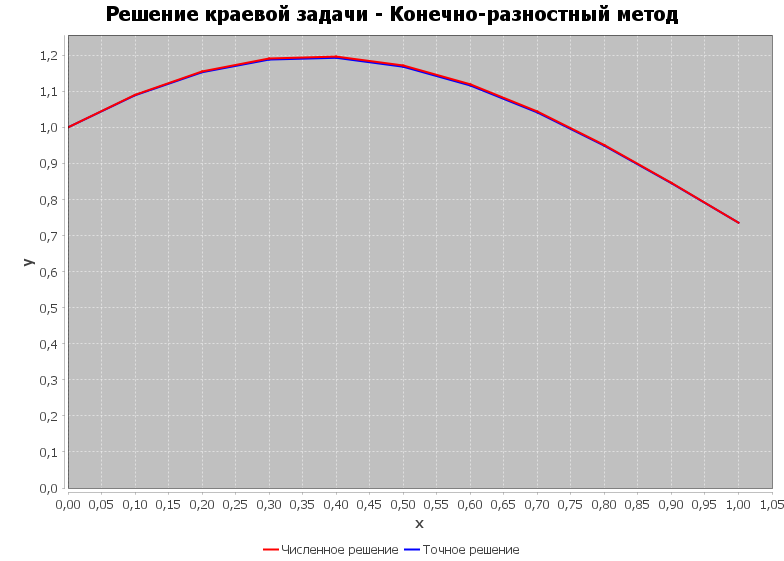
\includegraphics[scale=0.5]{chart1}

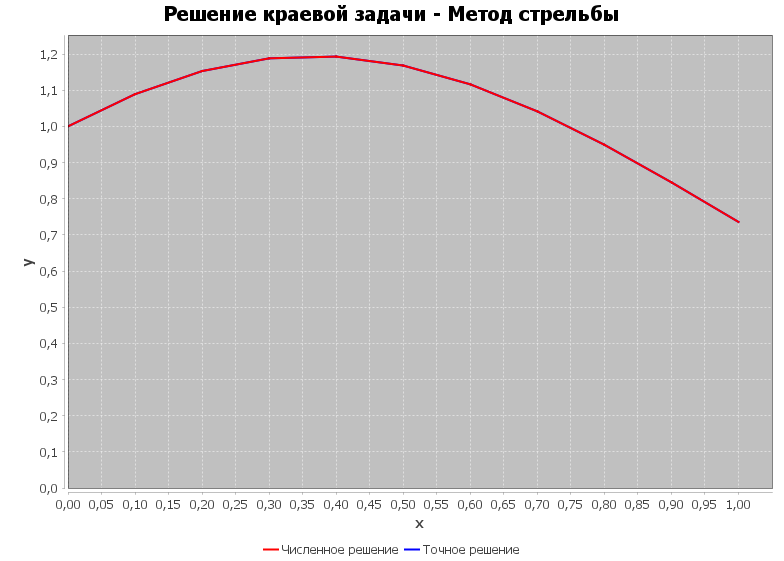
\includegraphics[scale=0.5]{chart2}

\pagebreak
